% Created by tikzDevice version 0.12.6 on 2024-03-01 18:55:41
% !TEX encoding = UTF-8 Unicode
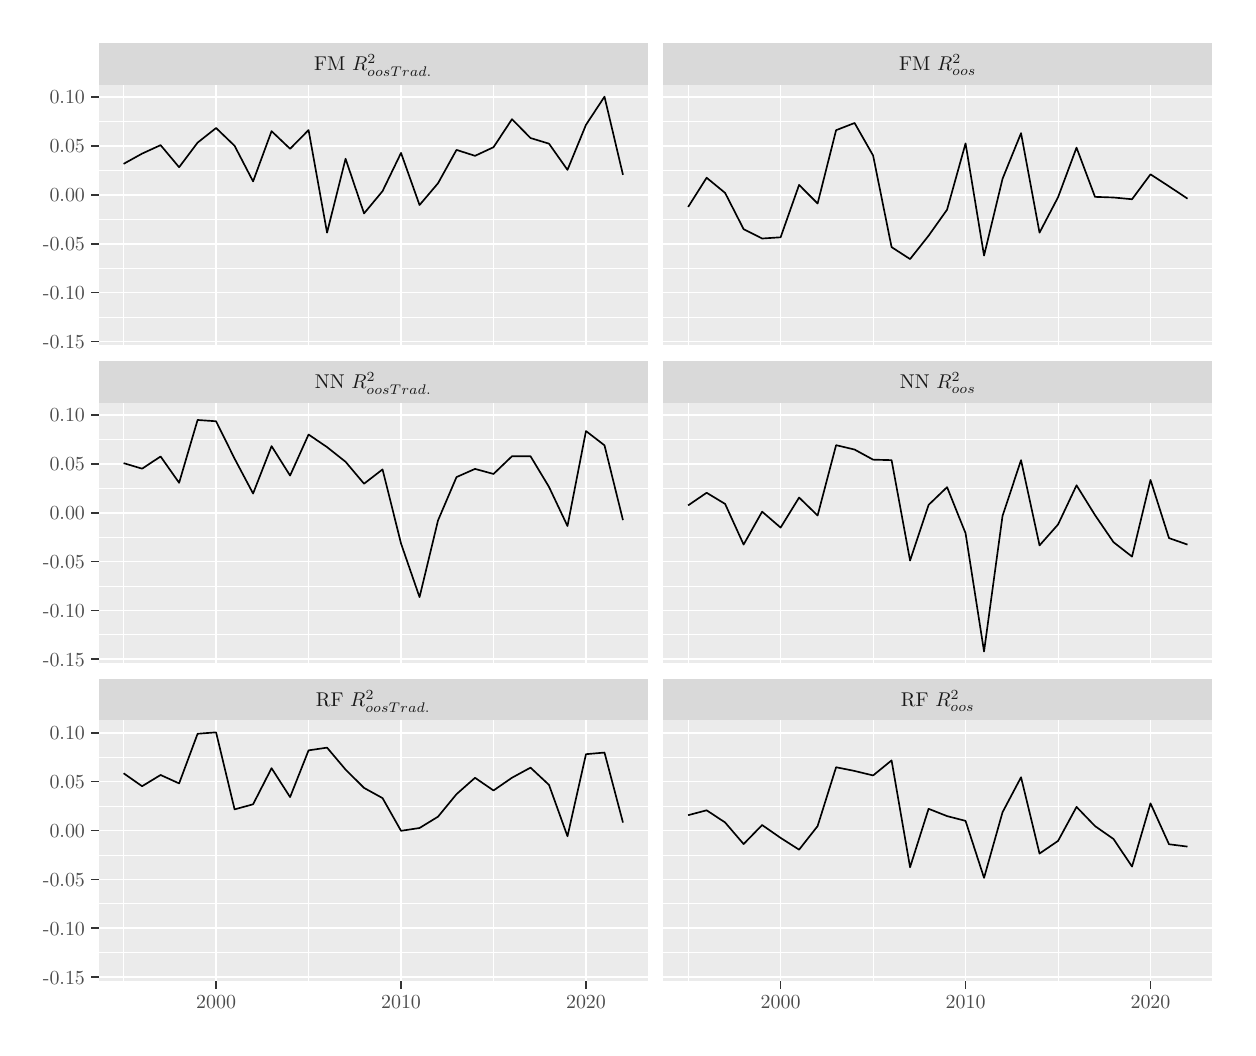
\begin{tikzpicture}[x=1pt,y=1pt]
\definecolor{fillColor}{RGB}{255,255,255}
\path[use as bounding box,fill=fillColor,fill opacity=0.00] (0,0) rectangle (433.62,361.35);
\begin{scope}
\path[clip] (  0.00,  0.00) rectangle (433.62,361.35);
\definecolor{drawColor}{RGB}{255,255,255}
\definecolor{fillColor}{RGB}{255,255,255}

\path[draw=drawColor,line width= 0.6pt,line join=round,line cap=round,fill=fillColor] (  0.00,  0.00) rectangle (433.62,361.35);
\end{scope}
\begin{scope}
\path[clip] ( 25.65,246.50) rectangle (224.13,340.69);
\definecolor{fillColor}{gray}{0.92}

\path[fill=fillColor] ( 25.65,246.50) rectangle (224.13,340.69);
\definecolor{drawColor}{RGB}{255,255,255}

\path[draw=drawColor,line width= 0.3pt,line join=round] ( 25.65,256.79) --
	(224.13,256.79);

\path[draw=drawColor,line width= 0.3pt,line join=round] ( 25.65,274.45) --
	(224.13,274.45);

\path[draw=drawColor,line width= 0.3pt,line join=round] ( 25.65,292.11) --
	(224.13,292.11);

\path[draw=drawColor,line width= 0.3pt,line join=round] ( 25.65,309.77) --
	(224.13,309.77);

\path[draw=drawColor,line width= 0.3pt,line join=round] ( 25.65,327.43) --
	(224.13,327.43);

\path[draw=drawColor,line width= 0.3pt,line join=round] ( 34.67,246.50) --
	( 34.67,340.69);

\path[draw=drawColor,line width= 0.3pt,line join=round] (101.50,246.50) --
	(101.50,340.69);

\path[draw=drawColor,line width= 0.3pt,line join=round] (168.33,246.50) --
	(168.33,340.69);

\path[draw=drawColor,line width= 0.6pt,line join=round] ( 25.65,247.96) --
	(224.13,247.96);

\path[draw=drawColor,line width= 0.6pt,line join=round] ( 25.65,265.62) --
	(224.13,265.62);

\path[draw=drawColor,line width= 0.6pt,line join=round] ( 25.65,283.28) --
	(224.13,283.28);

\path[draw=drawColor,line width= 0.6pt,line join=round] ( 25.65,300.94) --
	(224.13,300.94);

\path[draw=drawColor,line width= 0.6pt,line join=round] ( 25.65,318.60) --
	(224.13,318.60);

\path[draw=drawColor,line width= 0.6pt,line join=round] ( 25.65,336.26) --
	(224.13,336.26);

\path[draw=drawColor,line width= 0.6pt,line join=round] ( 68.08,246.50) --
	( 68.08,340.69);

\path[draw=drawColor,line width= 0.6pt,line join=round] (134.91,246.50) --
	(134.91,340.69);

\path[draw=drawColor,line width= 0.6pt,line join=round] (201.74,246.50) --
	(201.74,340.69);
\definecolor{drawColor}{RGB}{0,0,0}

\path[draw=drawColor,line width= 0.6pt,line join=round] ( 34.67,312.14) --
	( 41.35,315.84) --
	( 48.03,318.90) --
	( 54.72,310.92) --
	( 61.40,319.80) --
	( 68.08,325.09) --
	( 74.77,318.66) --
	( 81.45,305.79) --
	( 88.13,323.95) --
	( 94.82,317.58) --
	(101.50,324.35) --
	(108.18,287.28) --
	(114.87,313.97) --
	(121.55,294.22) --
	(128.23,302.28) --
	(134.91,316.08) --
	(141.60,297.26) --
	(148.28,305.13) --
	(154.96,317.18) --
	(161.65,315.04) --
	(168.33,318.15) --
	(175.01,328.28) --
	(181.70,321.47) --
	(188.38,319.43) --
	(195.06,309.96) --
	(201.74,326.24) --
	(208.43,336.40) --
	(215.11,308.16);
\end{scope}
\begin{scope}
\path[clip] ( 25.65,131.66) rectangle (224.13,225.84);
\definecolor{fillColor}{gray}{0.92}

\path[fill=fillColor] ( 25.65,131.66) rectangle (224.13,225.84);
\definecolor{drawColor}{RGB}{255,255,255}

\path[draw=drawColor,line width= 0.3pt,line join=round] ( 25.65,141.94) --
	(224.13,141.94);

\path[draw=drawColor,line width= 0.3pt,line join=round] ( 25.65,159.60) --
	(224.13,159.60);

\path[draw=drawColor,line width= 0.3pt,line join=round] ( 25.65,177.26) --
	(224.13,177.26);

\path[draw=drawColor,line width= 0.3pt,line join=round] ( 25.65,194.92) --
	(224.13,194.92);

\path[draw=drawColor,line width= 0.3pt,line join=round] ( 25.65,212.58) --
	(224.13,212.58);

\path[draw=drawColor,line width= 0.3pt,line join=round] ( 34.67,131.66) --
	( 34.67,225.84);

\path[draw=drawColor,line width= 0.3pt,line join=round] (101.50,131.66) --
	(101.50,225.84);

\path[draw=drawColor,line width= 0.3pt,line join=round] (168.33,131.66) --
	(168.33,225.84);

\path[draw=drawColor,line width= 0.6pt,line join=round] ( 25.65,133.11) --
	(224.13,133.11);

\path[draw=drawColor,line width= 0.6pt,line join=round] ( 25.65,150.77) --
	(224.13,150.77);

\path[draw=drawColor,line width= 0.6pt,line join=round] ( 25.65,168.43) --
	(224.13,168.43);

\path[draw=drawColor,line width= 0.6pt,line join=round] ( 25.65,186.09) --
	(224.13,186.09);

\path[draw=drawColor,line width= 0.6pt,line join=round] ( 25.65,203.75) --
	(224.13,203.75);

\path[draw=drawColor,line width= 0.6pt,line join=round] ( 25.65,221.41) --
	(224.13,221.41);

\path[draw=drawColor,line width= 0.6pt,line join=round] ( 68.08,131.66) --
	( 68.08,225.84);

\path[draw=drawColor,line width= 0.6pt,line join=round] (134.91,131.66) --
	(134.91,225.84);

\path[draw=drawColor,line width= 0.6pt,line join=round] (201.74,131.66) --
	(201.74,225.84);
\definecolor{drawColor}{RGB}{0,0,0}

\path[draw=drawColor,line width= 0.6pt,line join=round] ( 34.67,203.99) --
	( 41.35,201.99) --
	( 48.03,206.40) --
	( 54.72,196.89) --
	( 61.40,219.59) --
	( 68.08,219.12) --
	( 74.77,205.61) --
	( 81.45,193.01) --
	( 88.13,210.14) --
	( 94.82,199.50) --
	(101.50,214.33) --
	(108.18,209.78) --
	(114.87,204.48) --
	(121.55,196.56) --
	(128.23,201.73) --
	(134.91,174.95) --
	(141.60,155.57) --
	(148.28,183.30) --
	(154.96,198.95) --
	(161.65,201.91) --
	(168.33,200.08) --
	(175.01,206.49) --
	(181.70,206.48) --
	(188.38,195.40) --
	(195.06,181.26) --
	(201.74,215.59) --
	(208.43,210.43) --
	(215.11,183.40);
\end{scope}
\begin{scope}
\path[clip] ( 25.65, 16.81) rectangle (224.13,111.00);
\definecolor{fillColor}{gray}{0.92}

\path[fill=fillColor] ( 25.65, 16.81) rectangle (224.13,111.00);
\definecolor{drawColor}{RGB}{255,255,255}

\path[draw=drawColor,line width= 0.3pt,line join=round] ( 25.65, 27.09) --
	(224.13, 27.09);

\path[draw=drawColor,line width= 0.3pt,line join=round] ( 25.65, 44.75) --
	(224.13, 44.75);

\path[draw=drawColor,line width= 0.3pt,line join=round] ( 25.65, 62.41) --
	(224.13, 62.41);

\path[draw=drawColor,line width= 0.3pt,line join=round] ( 25.65, 80.07) --
	(224.13, 80.07);

\path[draw=drawColor,line width= 0.3pt,line join=round] ( 25.65, 97.73) --
	(224.13, 97.73);

\path[draw=drawColor,line width= 0.3pt,line join=round] ( 34.67, 16.81) --
	( 34.67,111.00);

\path[draw=drawColor,line width= 0.3pt,line join=round] (101.50, 16.81) --
	(101.50,111.00);

\path[draw=drawColor,line width= 0.3pt,line join=round] (168.33, 16.81) --
	(168.33,111.00);

\path[draw=drawColor,line width= 0.6pt,line join=round] ( 25.65, 18.26) --
	(224.13, 18.26);

\path[draw=drawColor,line width= 0.6pt,line join=round] ( 25.65, 35.92) --
	(224.13, 35.92);

\path[draw=drawColor,line width= 0.6pt,line join=round] ( 25.65, 53.58) --
	(224.13, 53.58);

\path[draw=drawColor,line width= 0.6pt,line join=round] ( 25.65, 71.24) --
	(224.13, 71.24);

\path[draw=drawColor,line width= 0.6pt,line join=round] ( 25.65, 88.90) --
	(224.13, 88.90);

\path[draw=drawColor,line width= 0.6pt,line join=round] ( 25.65,106.56) --
	(224.13,106.56);

\path[draw=drawColor,line width= 0.6pt,line join=round] ( 68.08, 16.81) --
	( 68.08,111.00);

\path[draw=drawColor,line width= 0.6pt,line join=round] (134.91, 16.81) --
	(134.91,111.00);

\path[draw=drawColor,line width= 0.6pt,line join=round] (201.74, 16.81) --
	(201.74,111.00);
\definecolor{drawColor}{RGB}{0,0,0}

\path[draw=drawColor,line width= 0.6pt,line join=round] ( 34.67, 91.92) --
	( 41.35, 87.25) --
	( 48.03, 91.31) --
	( 54.72, 88.26) --
	( 61.40,106.20) --
	( 68.08,106.72) --
	( 74.77, 78.88) --
	( 81.45, 80.72) --
	( 88.13, 93.76) --
	( 94.82, 83.32) --
	(101.50,100.20) --
	(108.18,101.19) --
	(114.87, 93.26) --
	(121.55, 86.64) --
	(128.23, 82.95) --
	(134.91, 71.13) --
	(141.60, 72.15) --
	(148.28, 76.24) --
	(154.96, 84.38) --
	(161.65, 90.29) --
	(168.33, 85.71) --
	(175.01, 90.32) --
	(181.70, 93.96) --
	(188.38, 87.73) --
	(195.06, 69.16) --
	(201.74, 98.82) --
	(208.43, 99.41) --
	(215.11, 74.12);
\end{scope}
\begin{scope}
\path[clip] (229.63,246.50) rectangle (428.12,340.69);
\definecolor{fillColor}{gray}{0.92}

\path[fill=fillColor] (229.63,246.50) rectangle (428.12,340.69);
\definecolor{drawColor}{RGB}{255,255,255}

\path[draw=drawColor,line width= 0.3pt,line join=round] (229.63,256.79) --
	(428.12,256.79);

\path[draw=drawColor,line width= 0.3pt,line join=round] (229.63,274.45) --
	(428.12,274.45);

\path[draw=drawColor,line width= 0.3pt,line join=round] (229.63,292.11) --
	(428.12,292.11);

\path[draw=drawColor,line width= 0.3pt,line join=round] (229.63,309.77) --
	(428.12,309.77);

\path[draw=drawColor,line width= 0.3pt,line join=round] (229.63,327.43) --
	(428.12,327.43);

\path[draw=drawColor,line width= 0.3pt,line join=round] (238.66,246.50) --
	(238.66,340.69);

\path[draw=drawColor,line width= 0.3pt,line join=round] (305.49,246.50) --
	(305.49,340.69);

\path[draw=drawColor,line width= 0.3pt,line join=round] (372.32,246.50) --
	(372.32,340.69);

\path[draw=drawColor,line width= 0.6pt,line join=round] (229.63,247.96) --
	(428.12,247.96);

\path[draw=drawColor,line width= 0.6pt,line join=round] (229.63,265.62) --
	(428.12,265.62);

\path[draw=drawColor,line width= 0.6pt,line join=round] (229.63,283.28) --
	(428.12,283.28);

\path[draw=drawColor,line width= 0.6pt,line join=round] (229.63,300.94) --
	(428.12,300.94);

\path[draw=drawColor,line width= 0.6pt,line join=round] (229.63,318.60) --
	(428.12,318.60);

\path[draw=drawColor,line width= 0.6pt,line join=round] (229.63,336.26) --
	(428.12,336.26);

\path[draw=drawColor,line width= 0.6pt,line join=round] (272.07,246.50) --
	(272.07,340.69);

\path[draw=drawColor,line width= 0.6pt,line join=round] (338.90,246.50) --
	(338.90,340.69);

\path[draw=drawColor,line width= 0.6pt,line join=round] (405.73,246.50) --
	(405.73,340.69);
\definecolor{drawColor}{RGB}{0,0,0}

\path[draw=drawColor,line width= 0.6pt,line join=round] (238.66,296.57) --
	(245.34,307.12) --
	(252.02,301.63) --
	(258.70,288.55) --
	(265.39,285.16) --
	(272.07,285.60) --
	(278.75,304.53) --
	(285.44,297.80) --
	(292.12,324.30) --
	(298.80,326.90) --
	(305.49,315.15) --
	(312.17,282.05) --
	(318.85,277.73) --
	(325.54,286.17) --
	(332.22,295.58) --
	(338.90,319.53) --
	(345.58,279.00) --
	(352.27,306.76) --
	(358.95,323.23) --
	(365.63,287.27) --
	(372.32,300.07) --
	(379.00,318.00) --
	(385.68,300.21) --
	(392.37,299.98) --
	(399.05,299.35) --
	(405.73,308.35) --
	(412.41,304.01) --
	(419.10,299.57);
\end{scope}
\begin{scope}
\path[clip] (229.63,131.66) rectangle (428.12,225.84);
\definecolor{fillColor}{gray}{0.92}

\path[fill=fillColor] (229.63,131.66) rectangle (428.12,225.84);
\definecolor{drawColor}{RGB}{255,255,255}

\path[draw=drawColor,line width= 0.3pt,line join=round] (229.63,141.94) --
	(428.12,141.94);

\path[draw=drawColor,line width= 0.3pt,line join=round] (229.63,159.60) --
	(428.12,159.60);

\path[draw=drawColor,line width= 0.3pt,line join=round] (229.63,177.26) --
	(428.12,177.26);

\path[draw=drawColor,line width= 0.3pt,line join=round] (229.63,194.92) --
	(428.12,194.92);

\path[draw=drawColor,line width= 0.3pt,line join=round] (229.63,212.58) --
	(428.12,212.58);

\path[draw=drawColor,line width= 0.3pt,line join=round] (238.66,131.66) --
	(238.66,225.84);

\path[draw=drawColor,line width= 0.3pt,line join=round] (305.49,131.66) --
	(305.49,225.84);

\path[draw=drawColor,line width= 0.3pt,line join=round] (372.32,131.66) --
	(372.32,225.84);

\path[draw=drawColor,line width= 0.6pt,line join=round] (229.63,133.11) --
	(428.12,133.11);

\path[draw=drawColor,line width= 0.6pt,line join=round] (229.63,150.77) --
	(428.12,150.77);

\path[draw=drawColor,line width= 0.6pt,line join=round] (229.63,168.43) --
	(428.12,168.43);

\path[draw=drawColor,line width= 0.6pt,line join=round] (229.63,186.09) --
	(428.12,186.09);

\path[draw=drawColor,line width= 0.6pt,line join=round] (229.63,203.75) --
	(428.12,203.75);

\path[draw=drawColor,line width= 0.6pt,line join=round] (229.63,221.41) --
	(428.12,221.41);

\path[draw=drawColor,line width= 0.6pt,line join=round] (272.07,131.66) --
	(272.07,225.84);

\path[draw=drawColor,line width= 0.6pt,line join=round] (338.90,131.66) --
	(338.90,225.84);

\path[draw=drawColor,line width= 0.6pt,line join=round] (405.73,131.66) --
	(405.73,225.84);
\definecolor{drawColor}{RGB}{0,0,0}

\path[draw=drawColor,line width= 0.6pt,line join=round] (238.66,188.73) --
	(245.34,193.29) --
	(252.02,189.25) --
	(258.70,174.57) --
	(265.39,186.46) --
	(272.07,180.70) --
	(278.75,191.56) --
	(285.44,185.07) --
	(292.12,210.49) --
	(298.80,208.90) --
	(305.49,205.25) --
	(312.17,205.07) --
	(318.85,168.80) --
	(325.54,188.90) --
	(332.22,195.31) --
	(338.90,178.66) --
	(345.58,135.94) --
	(352.27,184.97) --
	(358.95,205.06) --
	(365.63,174.27) --
	(372.32,181.82) --
	(379.00,195.98) --
	(385.68,185.21) --
	(392.37,175.42) --
	(399.05,170.22) --
	(405.73,197.93) --
	(412.41,176.91) --
	(419.10,174.56);
\end{scope}
\begin{scope}
\path[clip] (229.63, 16.81) rectangle (428.12,111.00);
\definecolor{fillColor}{gray}{0.92}

\path[fill=fillColor] (229.63, 16.81) rectangle (428.12,111.00);
\definecolor{drawColor}{RGB}{255,255,255}

\path[draw=drawColor,line width= 0.3pt,line join=round] (229.63, 27.09) --
	(428.12, 27.09);

\path[draw=drawColor,line width= 0.3pt,line join=round] (229.63, 44.75) --
	(428.12, 44.75);

\path[draw=drawColor,line width= 0.3pt,line join=round] (229.63, 62.41) --
	(428.12, 62.41);

\path[draw=drawColor,line width= 0.3pt,line join=round] (229.63, 80.07) --
	(428.12, 80.07);

\path[draw=drawColor,line width= 0.3pt,line join=round] (229.63, 97.73) --
	(428.12, 97.73);

\path[draw=drawColor,line width= 0.3pt,line join=round] (238.66, 16.81) --
	(238.66,111.00);

\path[draw=drawColor,line width= 0.3pt,line join=round] (305.49, 16.81) --
	(305.49,111.00);

\path[draw=drawColor,line width= 0.3pt,line join=round] (372.32, 16.81) --
	(372.32,111.00);

\path[draw=drawColor,line width= 0.6pt,line join=round] (229.63, 18.26) --
	(428.12, 18.26);

\path[draw=drawColor,line width= 0.6pt,line join=round] (229.63, 35.92) --
	(428.12, 35.92);

\path[draw=drawColor,line width= 0.6pt,line join=round] (229.63, 53.58) --
	(428.12, 53.58);

\path[draw=drawColor,line width= 0.6pt,line join=round] (229.63, 71.24) --
	(428.12, 71.24);

\path[draw=drawColor,line width= 0.6pt,line join=round] (229.63, 88.90) --
	(428.12, 88.90);

\path[draw=drawColor,line width= 0.6pt,line join=round] (229.63,106.56) --
	(428.12,106.56);

\path[draw=drawColor,line width= 0.6pt,line join=round] (272.07, 16.81) --
	(272.07,111.00);

\path[draw=drawColor,line width= 0.6pt,line join=round] (338.90, 16.81) --
	(338.90,111.00);

\path[draw=drawColor,line width= 0.6pt,line join=round] (405.73, 16.81) --
	(405.73,111.00);
\definecolor{drawColor}{RGB}{0,0,0}

\path[draw=drawColor,line width= 0.6pt,line join=round] (238.66, 76.78) --
	(245.34, 78.55) --
	(252.02, 74.15) --
	(258.70, 66.35) --
	(265.39, 73.22) --
	(272.07, 68.58) --
	(278.75, 64.32) --
	(285.44, 72.84) --
	(292.12, 94.11) --
	(298.80, 92.76) --
	(305.49, 91.14) --
	(312.17, 96.58) --
	(318.85, 57.97) --
	(325.54, 79.09) --
	(332.22, 76.45) --
	(338.90, 74.73) --
	(345.58, 54.13) --
	(352.27, 77.87) --
	(358.95, 90.49) --
	(365.63, 62.92) --
	(372.32, 67.48) --
	(379.00, 79.77) --
	(385.68, 72.84) --
	(392.37, 68.17) --
	(399.05, 58.21) --
	(405.73, 81.05) --
	(412.41, 66.28) --
	(419.10, 65.43);
\end{scope}
\begin{scope}
\path[clip] ( 25.65,111.00) rectangle (224.13,126.16);
\definecolor{fillColor}{gray}{0.85}

\path[fill=fillColor] ( 25.65,111.00) rectangle (224.13,126.16);
\definecolor{drawColor}{gray}{0.10}

\node[text=drawColor,anchor=base,inner sep=0pt, outer sep=0pt, scale=  0.72] at (124.89,116.10) {RF $R^2_{oos  Trad.}$};
\end{scope}
\begin{scope}
\path[clip] (229.63,111.00) rectangle (428.12,126.16);
\definecolor{fillColor}{gray}{0.85}

\path[fill=fillColor] (229.63,111.00) rectangle (428.12,126.16);
\definecolor{drawColor}{gray}{0.10}

\node[text=drawColor,anchor=base,inner sep=0pt, outer sep=0pt, scale=  0.72] at (328.88,116.10) {RF $R^2_{oos}$};
\end{scope}
\begin{scope}
\path[clip] ( 25.65,225.84) rectangle (224.13,241.00);
\definecolor{fillColor}{gray}{0.85}

\path[fill=fillColor] ( 25.65,225.84) rectangle (224.13,241.00);
\definecolor{drawColor}{gray}{0.10}

\node[text=drawColor,anchor=base,inner sep=0pt, outer sep=0pt, scale=  0.72] at (124.89,230.94) {NN $R^2_{oos  Trad.}$};
\end{scope}
\begin{scope}
\path[clip] (229.63,225.84) rectangle (428.12,241.00);
\definecolor{fillColor}{gray}{0.85}

\path[fill=fillColor] (229.63,225.84) rectangle (428.12,241.00);
\definecolor{drawColor}{gray}{0.10}

\node[text=drawColor,anchor=base,inner sep=0pt, outer sep=0pt, scale=  0.72] at (328.88,230.94) {NN $R^2_{oos}$};
\end{scope}
\begin{scope}
\path[clip] ( 25.65,340.69) rectangle (224.13,355.85);
\definecolor{fillColor}{gray}{0.85}

\path[fill=fillColor] ( 25.65,340.69) rectangle (224.13,355.85);
\definecolor{drawColor}{gray}{0.10}

\node[text=drawColor,anchor=base,inner sep=0pt, outer sep=0pt, scale=  0.72] at (124.89,345.79) {FM $R^2_{oos  Trad.}$};
\end{scope}
\begin{scope}
\path[clip] (229.63,340.69) rectangle (428.12,355.85);
\definecolor{fillColor}{gray}{0.85}

\path[fill=fillColor] (229.63,340.69) rectangle (428.12,355.85);
\definecolor{drawColor}{gray}{0.10}

\node[text=drawColor,anchor=base,inner sep=0pt, outer sep=0pt, scale=  0.72] at (328.88,345.79) {FM $R^2_{oos}$};
\end{scope}
\begin{scope}
\path[clip] (  0.00,  0.00) rectangle (433.62,361.35);
\definecolor{drawColor}{gray}{0.20}

\path[draw=drawColor,line width= 0.6pt,line join=round] ( 68.08, 14.06) --
	( 68.08, 16.81);

\path[draw=drawColor,line width= 0.6pt,line join=round] (134.91, 14.06) --
	(134.91, 16.81);

\path[draw=drawColor,line width= 0.6pt,line join=round] (201.74, 14.06) --
	(201.74, 16.81);
\end{scope}
\begin{scope}
\path[clip] (  0.00,  0.00) rectangle (433.62,361.35);
\definecolor{drawColor}{gray}{0.30}

\node[text=drawColor,anchor=base,inner sep=0pt, outer sep=0pt, scale=  0.72] at ( 68.08,  6.90) {2000};

\node[text=drawColor,anchor=base,inner sep=0pt, outer sep=0pt, scale=  0.72] at (134.91,  6.90) {2010};

\node[text=drawColor,anchor=base,inner sep=0pt, outer sep=0pt, scale=  0.72] at (201.74,  6.90) {2020};
\end{scope}
\begin{scope}
\path[clip] (  0.00,  0.00) rectangle (433.62,361.35);
\definecolor{drawColor}{gray}{0.20}

\path[draw=drawColor,line width= 0.6pt,line join=round] (272.07, 14.06) --
	(272.07, 16.81);

\path[draw=drawColor,line width= 0.6pt,line join=round] (338.90, 14.06) --
	(338.90, 16.81);

\path[draw=drawColor,line width= 0.6pt,line join=round] (405.73, 14.06) --
	(405.73, 16.81);
\end{scope}
\begin{scope}
\path[clip] (  0.00,  0.00) rectangle (433.62,361.35);
\definecolor{drawColor}{gray}{0.30}

\node[text=drawColor,anchor=base,inner sep=0pt, outer sep=0pt, scale=  0.72] at (272.07,  6.90) {2000};

\node[text=drawColor,anchor=base,inner sep=0pt, outer sep=0pt, scale=  0.72] at (338.90,  6.90) {2010};

\node[text=drawColor,anchor=base,inner sep=0pt, outer sep=0pt, scale=  0.72] at (405.73,  6.90) {2020};
\end{scope}
\begin{scope}
\path[clip] (  0.00,  0.00) rectangle (433.62,361.35);
\definecolor{drawColor}{gray}{0.30}

\node[text=drawColor,anchor=base east,inner sep=0pt, outer sep=0pt, scale=  0.72] at ( 20.70,245.48) {-0.15};

\node[text=drawColor,anchor=base east,inner sep=0pt, outer sep=0pt, scale=  0.72] at ( 20.70,263.14) {-0.10};

\node[text=drawColor,anchor=base east,inner sep=0pt, outer sep=0pt, scale=  0.72] at ( 20.70,280.80) {-0.05};

\node[text=drawColor,anchor=base east,inner sep=0pt, outer sep=0pt, scale=  0.72] at ( 20.70,298.46) {0.00};

\node[text=drawColor,anchor=base east,inner sep=0pt, outer sep=0pt, scale=  0.72] at ( 20.70,316.12) {0.05};

\node[text=drawColor,anchor=base east,inner sep=0pt, outer sep=0pt, scale=  0.72] at ( 20.70,333.78) {0.10};
\end{scope}
\begin{scope}
\path[clip] (  0.00,  0.00) rectangle (433.62,361.35);
\definecolor{drawColor}{gray}{0.20}

\path[draw=drawColor,line width= 0.6pt,line join=round] ( 22.90,247.96) --
	( 25.65,247.96);

\path[draw=drawColor,line width= 0.6pt,line join=round] ( 22.90,265.62) --
	( 25.65,265.62);

\path[draw=drawColor,line width= 0.6pt,line join=round] ( 22.90,283.28) --
	( 25.65,283.28);

\path[draw=drawColor,line width= 0.6pt,line join=round] ( 22.90,300.94) --
	( 25.65,300.94);

\path[draw=drawColor,line width= 0.6pt,line join=round] ( 22.90,318.60) --
	( 25.65,318.60);

\path[draw=drawColor,line width= 0.6pt,line join=round] ( 22.90,336.26) --
	( 25.65,336.26);
\end{scope}
\begin{scope}
\path[clip] (  0.00,  0.00) rectangle (433.62,361.35);
\definecolor{drawColor}{gray}{0.30}

\node[text=drawColor,anchor=base east,inner sep=0pt, outer sep=0pt, scale=  0.72] at ( 20.70,130.63) {-0.15};

\node[text=drawColor,anchor=base east,inner sep=0pt, outer sep=0pt, scale=  0.72] at ( 20.70,148.29) {-0.10};

\node[text=drawColor,anchor=base east,inner sep=0pt, outer sep=0pt, scale=  0.72] at ( 20.70,165.95) {-0.05};

\node[text=drawColor,anchor=base east,inner sep=0pt, outer sep=0pt, scale=  0.72] at ( 20.70,183.61) {0.00};

\node[text=drawColor,anchor=base east,inner sep=0pt, outer sep=0pt, scale=  0.72] at ( 20.70,201.27) {0.05};

\node[text=drawColor,anchor=base east,inner sep=0pt, outer sep=0pt, scale=  0.72] at ( 20.70,218.93) {0.10};
\end{scope}
\begin{scope}
\path[clip] (  0.00,  0.00) rectangle (433.62,361.35);
\definecolor{drawColor}{gray}{0.20}

\path[draw=drawColor,line width= 0.6pt,line join=round] ( 22.90,133.11) --
	( 25.65,133.11);

\path[draw=drawColor,line width= 0.6pt,line join=round] ( 22.90,150.77) --
	( 25.65,150.77);

\path[draw=drawColor,line width= 0.6pt,line join=round] ( 22.90,168.43) --
	( 25.65,168.43);

\path[draw=drawColor,line width= 0.6pt,line join=round] ( 22.90,186.09) --
	( 25.65,186.09);

\path[draw=drawColor,line width= 0.6pt,line join=round] ( 22.90,203.75) --
	( 25.65,203.75);

\path[draw=drawColor,line width= 0.6pt,line join=round] ( 22.90,221.41) --
	( 25.65,221.41);
\end{scope}
\begin{scope}
\path[clip] (  0.00,  0.00) rectangle (433.62,361.35);
\definecolor{drawColor}{gray}{0.30}

\node[text=drawColor,anchor=base east,inner sep=0pt, outer sep=0pt, scale=  0.72] at ( 20.70, 15.78) {-0.15};

\node[text=drawColor,anchor=base east,inner sep=0pt, outer sep=0pt, scale=  0.72] at ( 20.70, 33.44) {-0.10};

\node[text=drawColor,anchor=base east,inner sep=0pt, outer sep=0pt, scale=  0.72] at ( 20.70, 51.10) {-0.05};

\node[text=drawColor,anchor=base east,inner sep=0pt, outer sep=0pt, scale=  0.72] at ( 20.70, 68.76) {0.00};

\node[text=drawColor,anchor=base east,inner sep=0pt, outer sep=0pt, scale=  0.72] at ( 20.70, 86.42) {0.05};

\node[text=drawColor,anchor=base east,inner sep=0pt, outer sep=0pt, scale=  0.72] at ( 20.70,104.08) {0.10};
\end{scope}
\begin{scope}
\path[clip] (  0.00,  0.00) rectangle (433.62,361.35);
\definecolor{drawColor}{gray}{0.20}

\path[draw=drawColor,line width= 0.6pt,line join=round] ( 22.90, 18.26) --
	( 25.65, 18.26);

\path[draw=drawColor,line width= 0.6pt,line join=round] ( 22.90, 35.92) --
	( 25.65, 35.92);

\path[draw=drawColor,line width= 0.6pt,line join=round] ( 22.90, 53.58) --
	( 25.65, 53.58);

\path[draw=drawColor,line width= 0.6pt,line join=round] ( 22.90, 71.24) --
	( 25.65, 71.24);

\path[draw=drawColor,line width= 0.6pt,line join=round] ( 22.90, 88.90) --
	( 25.65, 88.90);

\path[draw=drawColor,line width= 0.6pt,line join=round] ( 22.90,106.56) --
	( 25.65,106.56);
\end{scope}
\end{tikzpicture}
